\chapter{Cinétique du réacteur ponctuel}
\section{Équation de cinétique ponctuelle}
\subsection{Introduction}
Nous avons eu du mal avec six variables, ça risque d'être pire si on ajoute le temps. Si il était 
possible de faire une sorte de séparation des variables, ça pourrait bien se simplifier
\begin{equation}
\varphi (\bar r,v,\bar \Omega ,t)\, \equiv \;T(t).\psi (\bar r,v,\bar \Omega )
\end{equation}
Ceci suppose que s'il y a des variations dans le temps la forme reste inchangée mais l'amplitude 
varie au cours du temps.  Hélas, ceci n'est possible que si $J,K$ sont constants ce qui n'est pas
réaliste. Cependant, une "fausse factorisation" peut être acceptable dans le cas où les perturbations 
n'affectent que peu la forme du flux autour de la criticité (une sorte de transitoire)
\begin{equation}
\varphi (\bar r,v,\bar \Omega ,t)\, \equiv \;T(t).\psi (\bar r,v,\bar \Omega ,t)
\end{equation}
où $T(t)$ est une fonction d'amplitude qui reprend les variations dépendantes du temps sur des temps
caractéristiques courts. Il y aura également une variation temporelle de $\psi$, mais plus lente. En 
bref, très rapidement on aura un facteur de multiplication du flux et puis, plus lentement, des 
changements dans le réacteur. Les barres avaleuses de neutrons correspondent à une telle situation.\\

Le raisonnement est le suivant
\begin{enumerate}
\item On utilise la factorisation \textit{partielle} $\varphi (\bar r,v,\bar \Omega ,t)\, \equiv \;T(t).
\psi (\bar r,v,\bar \Omega ,t)$  dans l'équation de Boltzmann avec les neutrons retardés (évidemment 
car ils dépendent du temps)(sans oublier la normalisation)
\item On regarde l'impact des hypothèses d'une factorisation \textit{exacte} $\varphi (\bar r,v,\bar \Omega ,t)\, \equiv \;T(t).\psi (\bar r,v,\bar \Omega )$
\begin{itemize}
\item[$\bullet$] Déduction d'un modèle d'évolution du réacteur sujet à des perturbations autour de
l'état stationnaire critique de régime
\item[$\bullet$] Solution exacte et approximée en fonction du type de perturbation
\end{itemize}
\end{enumerate}

\subsection{Déduction intuitive des équations ponctuelles}
\subsubsection{Évolution de la population neutronique sans neutrons et sources retardées}
Commençons par un peu d'intuition. Nous avions vu, au premier chapitre
\begin{equation}
\frac{{dN(t)}}{{dt}} = \frac{{{k_{eff}} - 1}}{\ell }N(t)
\end{equation}
où $l$ est la durée moyenne sur laquelle les neutrons sont consommés dans un cycle : nous avions 
un trop plein de neutrons qui donnait une ED avec une solution exponentielle ingérable, il était 
nécessaire d'introduire les neutrons retardés.\\

Considérons une fonction amplitude $T$ ($\propto N$) des neutrons retardés ainsi qu'une source 
indépendante
\begin{equation}
\frac{{dT(t)}}{{dt}} = \frac{{{k_{eff}}(1 - \beta ) - 1}}{\ell }T(t) + \sum\limits_{i = 1}^6    {\lambda _i}{c_i}(t) + q(t)
\end{equation}
où $c_i(t)$ est la concentration en précurseurs du groupe $i$. Le $(1-\beta)$ donne la fraction des neutrons prompts, le $-1$ l'éventuel surplus puis pomme il faut exprimer par cycle on divise par $l$
et on multiplie le tout par $T$. \\

Introduisons un autre temps caractéristique $\Lambda$ lié au $k_{eff}$ tel que $l=\Lambda k_{eff}$ 
ainsi que la \textbf{réactivité}, l'écart relatif de distance à la criticité
\begin{equation}
\rho  \equiv \frac{{{k_{eff}} - 1}}{{{k_{eff}}}}
\end{equation}
En substituant\footnote{Besoin de notes manuscrites}, on trouve
\begin{equation}
\frac{{dT(t)}}{{dt}} = \frac{{\rho  - \beta }}{\Lambda }T(t) + \sum\limits_{i = 1}^6   {\lambda _i}{c_i}(t) + q(t)
\end{equation}
Le seuil \textit{prompt-critique}\footnote{Notes manuscrites!} correspond au cas où la criticité est
obtenue \textbf{uniquement} avec des neutrons prompts soit le cas où $k_{eff}=(1-\beta)^{-1}$. En 
en tire
\begin{equation}
\rho = \beta
\end{equation}
En l'exprime en \%, pcm où en \$ (1\$ si $\rho = \beta$). \\

Tentons d'interpréter le temps caractéristique dans le cas mono-cinétique. On se rappelle que 
$\Sigma_a$ est la probabilité par unité de longueur d'avoir une interaction dans le libre 
parcours. Si on multiplie ce-dernier par la vitesse $v$, on aura la probabilité par unité de temps
d'avoir une absorption. Le temps moyen est bien l'inverse de cette grandeur et porte le nom de 
\textbf{temps de destruction}
\begin{equation}
\ell  = \frac{1}{{v{\Sigma _a}}}
\end{equation}
De façon similaire, $\frac{1}{v\Sigma_f}$ est le temps moyen pour avoir une fission. Si on divise 
ceci par le nombre de neutrons $\nu$, on trouve le temps moyen que met un neutron pour générer une 
fission, soit le \textbf{temps de production}
\begin{equation}
\Lambda  = \frac{1}{{\nu v{\Sigma _f}}}
\end{equation}
La criticité est atteinte si et seulement si $\Lambda=l$.


\subsection{Modèle du réacteur ponctuel}
Reprenons notre fonction amplitude
\begin{equation}
\frac{{dT(t)}}{{dt}} = \frac{{\rho \;\;\; - \beta }}{\Lambda }T(t) + \sum\limits_{i = 1}^6   {\lambda _i}{c_i}(t) + q(t)
\end{equation}
La concentration en précurseurs dans le groupe $i$ est donnée par
\begin{equation}
\frac{{d{c_i}(t)}}{{dt}} = \frac{{{\beta _i}}}{\Lambda }T(t) - {\lambda _i}{c_i}(t)
\end{equation}
Cette variation est constituée d'une diminution radioactive des précurseurs et d'une fraction 
$\beta_i$ qui se rajoute à cette concentration par cycle (on a bien une division par le temps de
production des neutrons): chaque fois que l'on a une contribution au flux, il y a une fraction
$\beta_i$ qui correspond aux neutrons retardés et donc les précurseurs du groupe correspondant 
(fragments). Ceci nous donne un système de $6+1=7$ équations. \\

Les variations de $T$ sont dues à des variations du flux causée par des variations de la puissance 
et donc des variations de températures. Nous avions jusqu'ici supposé que la vitesse des noyaux 
lourds était négligeable mais s'il y a une variation de la température du réacteur on va avoir une
nuance entre la vitesse absolue et relatives des neutrons et des noyaux lourds avec lesquels ils 
interagissent. Une variation de $T$ cause donc une variation de l'équation générale du réacteur car 
modifier le température de l'eau modifie sa densité impliquant un ralentissement des neutrons plus
ou moins important. \\

Tout ceci pour dire que $T$ varie, on aura un effet sur la réactivité (car écart par rapport à 
l'équilibre). Le problème devient linéaire et pour tenir compte de ceci un suppose une réactivité
dépendante du temps mais extérieure\footnote{On néglige la rétroaction et on voit $\rho(t)$ comme 
un signal extérieur.} : $\rho\to\rho(t)$.

\subsection{Solution des équations cinétiques ponctuelles pour une marche de réactivité}
\subsubsection{Problématique}
On s'intéresse au déplacement rapide en $t=0$ des barres de commande dans un réacteur initialement
stable et critique sans source
\begin{equation}
\left\{ {\begin{array}{*{20}{c}}
{\rho (t) = 0}&{,\;t < 0}\\
{\rho (t) = \rho }&{,\;t \ge 0}
\end{array}} \right.
\end{equation}
Il faut résoudre nous deux équations différentielles de $\dot{T}$ et $\dot{c}$. En effectuant 
la transformée de Laplace\footnote{Notes manuscrites!}
\begin{equation}
\left\{\begin{array}{ll}
\bar T(p) &\DS= \frac{{\Lambda (T(0) + \sum\nolimits_i    {\textstyle{{{\lambda _i}{c_i}(0)} \over {p + {\lambda _i}}}})}}{{\Lambda p - \rho  + \sum\nolimits_i    {\textstyle{{{\beta _i}p} \over {p + {\lambda _i}}}}}}\\
{\bar c_i}(p) &\DS= \frac{{{\textstyle{{{\beta _i}} \over \Lambda }}\bar T(p) + {c_i}(0)}}{{p + {\lambda _i}}}
\end{array}\right.
\end{equation}
Avec comme $\DS CI\; \to \;\left( {{\lambda _i}{c_i}(0) = \frac{{{\beta _i}}}{\Lambda }T(0)} \right)$. 
Introduisons une fonction $1/G$ car on retrouve celle-ci de chaque côté de l'égalité à $p$ près\footnote{Il faudrait des notes pour éclaircir ces opérations}
\begin{equation}
{[G(p)]^{ - 1}} \equiv p\left(   \right.1 + \frac{1}{\Lambda }\sum\limits_i    \frac{{{\beta _i}}}{{p + {\lambda _i}}}\left.    \right)
\end{equation}
Ce qui permet d'écrire\\
	\begin{wrapfigure}[5]{l}{5cm}
	\vspace{-5mm}
	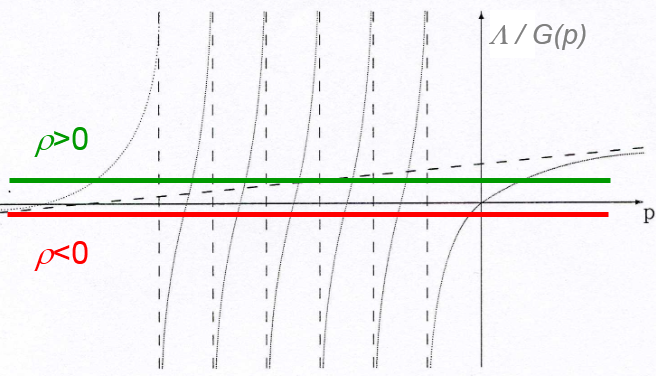
\includegraphics[scale=0.23]{ch5/image1.png}
	\captionof{figure}{ }
	\end{wrapfigure}
\cadre{
\begin{equation}
\frac{{\bar T(p)}}{{T(0)}} = \frac{1}{{p[1 - {\textstyle{\rho  \over \Lambda }}G(p)]}}
\end{equation}}\ \\

Il s'agit d'une expression donnant sept pôles possibles. Le pôle dominant donne le comportement 
dominant. Pour $\rho >0$ le pôle dominant est positif alors qu'il est négatif pour $\rho<0$.\vspace{3mm}


\subsubsection{Inversion de $\bar T(p)$}
Identifions les pôles, soit les racines de $\rho =\dfrac{\Lambda}{G(p)}$. Notons que $p=0$ n'est 
pas un pôle s'il n'y a pas de source. Nous avions vu avec l'illustration ci-dessus qu'il y avait
sept pôles
\begin{itemize}
\item[$\bullet$] $\rho<0$ : 7 pôles.
\item[$\bullet$] $\rho>0$ : 6 pôles négatif et un positif $\to p_0>0>p_1>\dots > p_6$.
\end{itemize}\ 

Tout dans ce problème est connu, par calcul des résidus il est possible de calculer les valeurs 
exactes des écarts. Dans notre cas, on s'intéresse au pôle qui a la plus grande valeur (le plus loin
sur l'axe $p$) car l'inverse de ce pôle en valeur absolue donnera le temps caractéristique 
apparaissant dans l'exponentielle dominante (comportement en $e^{\pm t/\tau)}$ que le réacteur va
suivre pour cet échelon de réactivité
\begin{equation}
T(t) = \sum\limits_{k = 0}^6    {T_k}{e^{{p_k}t}}\quad\overset{t\to\infty}{\longrightarrow}\quad {T_o}{e^{{p_o}t}}
\end{equation}
où $\DS \frac{{{T_k}}}{{T(0)}} = \mathop {\lim }\limits_{p \to {p_k}} \frac{{p - {p_k}}}{{p[1 - {\textstyle{\rho  \over \Lambda }}G(p)]}} = \frac{1}{{1 - {\textstyle{\rho  \over \Lambda }}(G({p_k}) + {p_k}G'({p_k}))}}  = \frac{{1 + \frac{1}{\Lambda }\sum\limits_i    \frac{{{\beta _i}}}{{{p_k} + {\lambda _i}}}}}{{1 + \frac{1}{\Lambda }\sum\limits_i   \frac{{{\beta _i}{\lambda _i}}}{{{{({p_k} + {\lambda _i})}^2}}}}}$.\\

La période asymptotique du réacteur est donc donnée par $\tau = 1/|p_0|$. On en tire une relation
\textit{période-réactivité} qui porte le doux nom d'\textbf{équation inhour}\\

\cadre{\begin{equation}
\rho  = \frac{\Lambda }{{G(1/\tau )}}
\end{equation}}\ \\

A l'aide de cette équation, il est possible en mesurant le temps nécessaire $\tau$ pour une variation
du flux d'en déduire $\rho$, par exemple liée à la descente des barres de contrôles d'un coup dans 
le réacteur. Il s'agit du temps nécessaire pour que le flux varie d'un facteur $e$ en croissance ou en
décroissance selon le signe de la réactivité.

\subsubsection{Cas limites}
Reprenons l'équation inhour en écrivant celle-ci par rapport à la période et non plus par rapport 
à $p$
\begin{equation}
\rho  \equiv \frac{\Lambda }{\tau }\left(    1 + \frac{1}{\Lambda }\sum\limits_i    \frac{{{\beta _i}\tau }}{{1 + {\lambda _i}\tau }}    \right)
\end{equation}
En se rappelant que $\beta$ est le seuil prompt-critique, voyons trois cas limites
\begin{enumerate}
\item \textit{Grande réactivité} : $\rho > \beta \to \lambda_i\tau \ll 1$. Ceci signifie que la 
période est très petite par rapport au $1/\lambda_i$ soit le temps de vie des précurseurs : les
$\lambda_i\tau$ peuvent être négligés dans l'équation inhour
\begin{equation}
\rho  \equiv \frac{\Lambda }{\tau }\left(   1 + \frac{1}{\Lambda }\sum\limits_i    \frac{{{\beta _i}\tau }}{{1 + {\lambda _i}\tau }}    \right)\overset{\lambda_i\tau\ll 1}{\longrightarrow}  \frac{\Lambda }{\tau } + \beta \qquad\Rightarrow\qquad \tau\longrightarrow \frac{\Lambda }{{\rho  - \beta }}
\end{equation}
Le temps ne dépend en aucune manière des $\lambda_i$ (invese des temps caractéristiques des neutrons
retardés). Ainsi, au dessus du seuil prompt-critique, la période asymptotique dépend de $\Lambda$ mais
(encore une fois) pas des $1/\lambda_i$ qui sont lié (à $\ln 2$ près) à la demi-vie des précurseurs. 
L'agrandissement du flux $\varphi$ est trop rapide pour que les neutrons retardés puissent jouer un rôle au dessus du seuil prompt-critique donné par $k_{eff}(1-\beta)=1$.

\item \textit{Petite réactivité} : $0<\rho\ll \beta \to \lambda_i\tau \gg 1$. Ceci signifie que 
$\rho$ se rapproche à l'horizontale à zéro et donc la valeur du pôle dominant est petite impliquant
une période grande.  Avec cette approximation, c'est le 1 dans le dénominateur de l'équation inhour 
que l'on négliger. Cette simplification permet de simplifier les $\tau$ dans la fraction
\begin{equation}
\rho  \equiv \frac{\Lambda }{\tau }\left(    1 + \frac{1}{\Lambda }\sum\limits_i    \frac{{{\beta _i}\tau }}{{1 + {\lambda _i}\tau }}    \right)\overset{\lambda_i\tau\gg1}{\longrightarrow}  \frac{1}{\tau }(\Lambda  + \beta \bar \tau )
\end{equation}
Comme précédemment, $1/\lambda_i$ est le temps de demi-vie des précurseur : on fait apparaître un 
temps moyen $\bar\tau$ car la sommation ne faut que pondérer les $1/\lambda_i$ par $\beta_i/\beta$.
\begin{equation}
\bar \tau  \equiv \sum\limits_i    \frac{{{\beta _i}/\beta }}{{{\lambda _i}}}
\end{equation}
Il s'agit donc du temps de vie moyen des neutrons retardés pondéré par leur fraction relative. Notons
que cette expression est indépendante de $\Lambda$. Ici, ce sont les neutrons retardés qui commandent
la croissance du flux $\varphi$ comme nous l'avions déduit intuitivement au premier chapitre. 

\item \textit{Réactivité <0}. Il y a un pôle dominant entre 0 et $\lambda_1$ qui est le pôle le plus
petit en valeur absolue. La période est plus grande que le temps caractéristique le plus grand des 
demi-vie des neutrons retardés, il en résulte un écrasement de la valeur du flux liée au temps 
caractéristique des neutrons retardés
\begin{equation}
\tau  > 1/{\lambda _1}
\end{equation}
\end{enumerate}


\subsubsection{Modèle ponctuel à un groupe de neutrons retardés}
Nos deux équations à résoudre sont
\begin{equation}
\frac{{dT(t)}}{{dt}} = \frac{{\rho (t) - \beta }}{\Lambda }T(t) + \lambda c(t),\qquad\qquad
\frac{{dc(t)}}{{dt}} = \frac{\beta }{\Lambda }T(t) - \lambda c(t)
\end{equation}
En dérivant $dT/dt$ on fait apparaître $dc/dt$ et on peut y substituer la seconde équation\footnote{Notes manuscrites!!}. On se retrouve alors avec une équation qui où n'apparaît que $T$. En 
faisant la résolution de cette équation (solutions exponentielles ou partir de l'équation inhour 
à un seul groupe) on trouve une équation du second degré en $p$ donnant les pôles
\begin{equation}
\rho  \equiv \Lambda p\left(   \right.1 + \frac{1}{\Lambda }\frac{\beta }{{p + \lambda }}\left.    \right)
\end{equation}
Après résolution 
\begin{equation}
\left. {\begin{array}{*{20}{c}}
{{\omega _1}}\\
{{\omega _2}}
\end{array}} \right\} =  - \frac{{\beta  - \rho  + \lambda \Lambda  \pm \sqrt {{{(\beta  - \rho  + \lambda \Lambda )}^2} + 4\lambda \Lambda \rho } }}{{2\Lambda }}\quad\overset{{\lambda \Lambda  \ll \beta  - \rho }}{\longrightarrow} \quad
\left\{ {\begin{array}{*{20}{c}}
\DS{{\omega _1} =  - \frac{{\beta  - \rho }}{\Lambda }}\vspace{2mm}\\
\DS{{\omega _2} = \frac{{\lambda \rho }}{{\beta  - \rho }}}
\end{array}} \right.
\end{equation}
Après calcul, on se retrouve avec une combinaison linéaire d'exponentielles
\begin{equation}
T(t) \cong \frac{{T(0)}}{{\beta  - \rho }}\left[ {\beta \exp \left( {\frac{{\lambda \rho }}{{\beta  - \rho }}t} \right)} \right. - \rho \exp \left. {\left( { - \frac{{\beta  - \rho }}{\Lambda }t} \right)} \right]
\label{eq:Ch5.1}
\end{equation}
Le premier terme donne le comportement asymptotique et le second le transitoire rapidement amorti. Le 
slide 12 donne des cas de transitoires possibles mais n'ayant que peu de notes\footnote{A rajouter} 
je ne le mets pas ici.


\section{Solutions approximées pour une réactivité dépendante du temps}
\subsection{Énoncé du problème}
La solution exacte du modèle du réacteur ponctuel n'est possible que pour un step de réactivité via 
l'équation inhour. Pour les autres cas il faut recourir au calcul numérique ou via des approximations
\begin{itemize}
\item[$\bullet$] Le transitoire est long par rapport au temps de génération des neutrons prompts
\begin{itemize}
\item[$\to$] Gouvernance par les neutrons retardés : \textit{approximation du saut prompt}
\end{itemize}
\item[$\bullet$] Le transitoire est très rapide, fortement au dessus du seuil prompt-critique
\begin{itemize}
\item[$\to$] Effet des neutrons prompts seulement : \textit{approximation prompt}
\end{itemize}
\end{itemize}


\subsection{Approximation du saut prompt}
Ici le transitoire est lent, le temps de production des neutrons tend à s'annuler : $\Lambda\to0$. 
Ceci signifie que le temps caractéristique du transitoire est très supérieur à $\Lambda$ et donc le
transitoire est gouverné par les neutrons retardé. Nous allons considéré un développement en série 
de la fonction amplitude $T(t)$ par rapport au paramètre $\Lambda$ et voir ce qui se passe aux
premiers ordres\footnote{Voir notes manuscrites}
\begin{equation}
T(t) = \sum\limits_{k = 0}^\infty    {\Lambda ^k}{T_k}(t)
\end{equation}
En partant de l'expression vue précédemment de $\frac{dT(t)}{dt}$ et en la dérivant, nous pouvons
obtenir
\begin{equation}
\dfrac{d^2T(t)}{dt^2} - \dfrac{dT(t)}{dt}\left[\frac{\rho(t)-\beta}{\Lambda}-\lambda\right]-\frac{\dot \rho(t)+\lambda\rho(t)}{\Lambda}T(t)=0
\end{equation}
Multiplions celle-ci par $\Lambda$
\begin{equation}
\Lambda \frac{{{d^2}T}}{{d{t^2}}} + (\beta  - \rho (t) + \lambda \Lambda )\frac{{dT}}{{dt}} - (\lambda \rho (t) + \dot \rho (t))T = 0
\end{equation}
Dans la limite où $\Lambda\to0$
\begin{equation}
(\beta  - \rho (t) )\frac{{dT}}{{dt}} - (\lambda \rho (t) + \dot \rho (t))T = 0
\end{equation}
En remplaçant $T(t)$ par son développement à l'ordre 0 en $\Lambda$\footnote{Revoir.}
\begin{equation}
\frac{{d{T_o}(t)}}{{dt}} = \frac{{(\lambda \rho (t) + \dot \rho (t))}}{{\beta  - \rho (t)}}{T_o}(t)
\end{equation}
Après résolution
\begin{equation}
{T_o}(t) = T(0).\exp \left. {\left[ {\int_o^t   \frac{{\lambda \rho (t')}}{{\beta  - \rho (t')}}dt'} \right.} \right].\frac{{\beta  - \rho (0)}}{{\beta  - \rho (t)}}
\end{equation}
Venons-en à l'esprit physique. Lorsque l'on applique l'approximation d'un échelon à quelque chose, 
cela symbolise quelque chose qui se passe assez rapidement : une sorte de $(1-\exp)$ rapide approchée
par l'échelon. On travaille donc avec un échelon qui est une montée exponentielle et le temps 
caractéristique est très grande devant $\Lambda$.\\

Tout ce que nous avons effectué ici en considérant qu'on se trouve après $t=0$ sur une réactivité 
constante (plateau de l'échelon) donne cette exponentielle. Il s'agit du terme dominant du 
comportement asymptotique que l'on avait sur l'échelon avec un groupe de neutrons retardés donné 
par \eqref{eq:Ch5.1} (le second terme s'amorti très vite car tout ce qui est de l'ordre de 
$\Lambda$ est négligé). Par contre on retrouve une discontinuité à l'origine, cachée par cette 
montée rapide. Cette discontinuité de la réactivité (due à l'échelon) justifie le saut $\dfrac{
\beta}{\beta-\rho}$ que nous avions en \eqref{eq:Ch5.1}.\\

Il faut que la borne de l'intégrale soit suffisamment faible et $\rho$ ne doit pas pouvoir dépasser
$\beta$ ce qui causerait un renversement du signe (le terme dominant et amorti s'échangeraient). 
Ce renversement de signe est cependant nécessaire si l'on souhaite que les neutrons retardés 
réagissent sinon ils seront rapidement amortis. Les slides 15-16 donnent des exemples et le slide 
18 a été passé.



\subsection{Approximation prompt}
Étudions le transitoire au dessus du seuil prompt-critique (on parle de \textit{superprompt}). On peut
négliger les neutrons retardés (une fois que $\rho(t)>\beta$)
\begin{equation}
\frac{{dT(t)}}{{dt}} = \frac{{\rho (t) - \beta }}{\Lambda }T(t)\qquad\Leftrightarrow\qquad
T(t) = {T_o}.\exp \left( {\int_o^t    \frac{{\rho (t') - \beta }}{\Lambda }dt'} \right)
\end{equation}
avec $T_0$ via $\rho(T_0)\geq \beta$ dans le calcul de $T(0)$. 

\subsubsection{Step}
Soit un step
\begin{equation}
\rho(t) = \rho.\theta(t),\qquad\rho>\beta
\end{equation}
On obtient $T_0$ avec le modèle à un groupe de neutrons retardés pour des transitoires très rapides
\begin{equation}
{T_o} = \frac{\rho }{{\rho  - \beta }}T(0),\qquad\qquad T(t) = {T_o}.\exp \left( {\frac{{\rho  - \beta }}{\Lambda }t} \right)
\end{equation}

\subsubsection{Rampe}
Soit une rampe
\begin{equation}
\rho(t) = at
\end{equation}
Comme le transitoire va très vite, la concentration en précurseur n'a pas le temps d'évaluer. Une 
façon de traiter cette approximation est de dire que le $c(t)$ présent dans le terme $\lambda c(t)$
est remplacé par $c_0$ (donné par la condition initiale, on reste en équilibre sur la concentration 
en précurseur sur un transitoire aussi rapide). Après quelques calculs qui ont été passés, il est 
possible d'obtenir
\begin{equation}
T(t) = {T_{pc}}.\exp \left( {\int_{{t_p}}^t   \frac{{at' - \beta }}{\Lambda }dt'} \right)
\end{equation}
\danger\ Il ne faut pas utiliser ce résultat sur quelque chose de non-prompt car la fonction 
amplitude décroit alors qu'elle devrait, dans ce cas la, augmenter.